\documentclass[11pt,reqno,final]{amsart}

\pdfcompresslevel=0
\pdfobjcompresslevel=0

\usepackage[dvipsnames]{xcolor}% adds colors
\usepackage{amsmath, amsthm}% {amsfonts, amssymb}

% New Characters
\usepackage[latin1]{inputenc}%
\usepackage[T1]{fontenc}

\usepackage{MnSymbol}
\usepackage[normalem]{ulem}% underlining

\usepackage[theoremfont, largesc]{newpxtext} % different text,math font
\usepackage{newpxmath}

\makeatletter
\DeclareMathRadical{\sqrtsign}{symbols}{112}{largesymbols}{112}
% \let\sqrt=\undefined
% \DeclareRobustCommand\sqrt{\@ifnextchar[\@sqrt{\mathpalette\@x@sqrt}]}
% \def\@x@sqrt#1#2{%
%  \setbox\z@\hbox{$\m@th#1\sqrtsign{\mkern1mu #2}$}
%  \mkern3mu\box\z@}
\makeatother




% Page Typesetting
\usepackage[final]{microtype}
\usepackage{relsize}
\usepackage[margin=1in]{geometry}
\usepackage{framed}
\usepackage{tikz}

\usepackage{csquotes}

\usepackage{setspace}
\onehalfspacing

\usepackage{hyperref}
\hypersetup{
  final,
  pdftitle={Math 135 - Second Derivative Test},
  pdfauthor={Bonventre}, 
  linktoc=page,
  pagebackref,
  colorlinks=true,
  citecolor=PineGreen,
  linkcolor=PineGreen,
  linkbordercolor=PineGreen,
}


% Internal References

\usepackage[inline,shortlabels]{enumitem}

% \numberwithin{equation}{section} 
\numberwithin{figure}{section}

\usepackage[nameinlink,capitalise,noabbrev]{cleveref}

\crefname{equation}{}{} % get \cref to behave as \eqref

% \theoremstyle{plain} % bold name, italic text
\newtheorem{theorem}[equation]{Theorem}%
\newtheorem*{theorem*}{Theorem}%
\newtheorem{lemma}[equation]{Lemma}%
\newtheorem{proposition}[equation]{Proposition}%
\newtheorem{corollary}[equation]{Corollary}%
\newtheorem{conjecture}[equation]{Conjecture}%
\newtheorem*{conjecture*}{Conjecture}%
\newtheorem{claim}[equation]{Claim}%
\newtheorem{question}{Question}

\theoremstyle{definition} % bold name, plain text
\newtheorem{definition}[equation]{Definition}%
\newtheorem*{definition*}{Definition}%
\newtheorem{example}[equation]{Example}%
\newtheorem*{example*}{Example}%
\newtheorem{remark}[equation]{Remark}%
\newtheorem{notation}[equation]{Notation}%
\newtheorem{convention}[equation]{Convention}%
\newtheorem{assumption}[equation]{Assumption}%
\newtheorem{exercise}[question]{Exercise}

% ---------- macros
\newcommand{\set}[1]{\left\{#1\right\}}%
\newcommand{\sets}[2]{\left\{ #1 \;|\; #2\right\}}%
\newcommand{\longto}{\longrightarrow}%
\newcommand{\into}{\hookrightarrow}%
\newcommand{\onto}{\twoheadrightarrow}%

\usepackage{harpoon}
\newcommand{\vect}[1]{\text{\overrightharp{\ensuremath{#1}}}}

\newcommand{\del}{\partial}%

\newcommand{\ki}{\chi}
\newcommand{\ksi}{\xi}
\newcommand{\Ksi}{\Xi}

\newcommand{\dlim}{\displaystyle\lim}

% %%%%%%%%%%%%%%%%%%%%%%%%%%%%%%%%%%%%%%%%%%%%%%%%%%%%%%%%%%%%%%%%%%%%%%%%%%%%%%%%%%%%%%%%%%%%%%%%%%%%

\begin{document}


\begin{center}
        \textbf{\Large Math 135, Calculus 1, Fall 2020}\\[10pt]
        {\large 11-13: Second Derivative Test (Section 4.4)}
\end{center}

\thispagestyle{empty}


\renewcommand{\thesection}{\Alph{section}}

% \vspace{-1pt}

The \textbf{derivative} $f'(x)$ of a function $y=f(x)$ gives:
\begin{itemize}
\item the slope of the tangent line
\item the instantaneous rate of change of $y$ with respect to $x$
\end{itemize}

In today's class we'll see how the second derivative yields information about the original function.

\section{Concavity}

The first derivative says whether the original function $f(x)$ is \textbf{increasing} or \textbf{decreasing}.
The second derivative talks about the \textit{curvature}, in particular the \textbf{concavity}, of the graph.
\begin{center}
        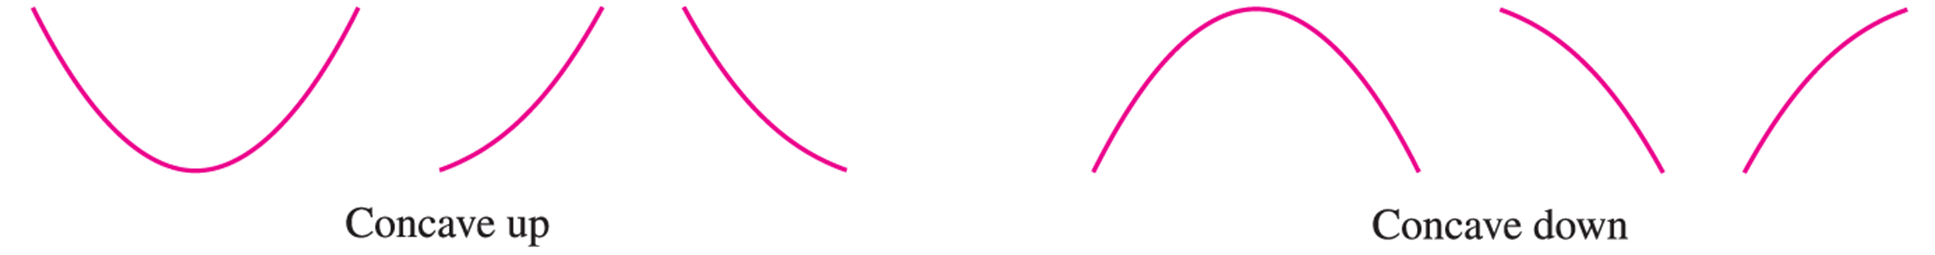
\includegraphics[width=\textwidth]{11-16P_concave}
\end{center}
\begin{framed}
        \begin{gather*}
                \mbox{$f''(x) > 0$ for $x \in (a,b)$
                  $\Rightarrow$
                  $f$ is \textbf{concave up} on $(a,b)$
                  $\Rightarrow$
                  the \textit{slope} is \textbf{increasing} on $(a,b)$
                }\\
                \mbox{$f''(x) < 0$ for $x \in (a,b)$
                  $\Rightarrow$
                  $f$ is \textbf{concave down} on $(a,b)$
                  $\Rightarrow$
                  the \textit{slope} is \textbf{decreasing} on $(a,b)$
                }
        \end{gather*}
\end{framed}

An \textbf{inflection point} $x = c$ is a point where the concavity \textit{changes}:
\begin{itemize}
\item $f''(c) = 0$, and
\item the sign of $f''$ flipes on either side of $x = c$.
\end{itemize}
\subsection*{Warning.} An \textit{inflection point} corresponds to the notion of a \textit{local extremum}, \textbf{not} a critical point!

\begin{example}
        Together, let's find the inflection points of the function $f(x) = (x-2)^3$.
        We will first find the intervals where $f$ is concave up and down.
        \vfill
\end{example}

\newpage

\begin{exercise}
        Let $g(x) = x^4 - 4x^3$. Find all inflection points.
        \vfill
        \vfill
\end{exercise}

\section{Second Derivative Test}

The second derivative can also be used to classify critical points:
\subsection*{Second Derivative Test}
Suppose that $x = c$ is a critical point of $f$.
\begin{framed}
        \begin{gather*}
                f''(c) > 0 \quad  \Rightarrow \quad \mbox{$c$ is a local min}\\
                f''(c) < 0 \quad \Rightarrow \quad \mbox{$c$ is a local max}\\
                f''(c) = 0 \quad \Rightarrow \quad \mbox{the test is \textbf{inconclusive}}
        \end{gather*}
\end{framed}
If the test is inconclusive, $x = c$ can be a local max, a local min, or neither!

\begin{exercise}
        Consider the function $f(x) = \dfrac{1}{x^2-x+2}$.
        \begin{enumerate}[(a)]
        \item Find and simplify $f'(x)$ and $f''(x)$.
                \vfill
        \item Find the critical points of $f$.
                \vfill
        \item Use the second derivative test to classify the critical points.
                \vfill
        \end{enumerate}
\end{exercise}

\newpage

\begin{exercise}
        Consider the function $h(x) = \sin x + \frac{x}{2}$ on the interval $[0,2\pi]$.
        Restricted to this interval,
        find all critical points, intervals of increase and decrease, intervals of concave up and concave down, and all inflection points. Classify all critical points.
        Use this information, as well as the function value at the critical points and inflection points,
        to sketch a graph of $h(x)$ on $[0, 2\pi]$.
\end{exercise}

\end{document}
